\documentclass[twoside]{report}

%%%%% ADDED TO SUPPORT TT BOLD FACES %%%%
\DeclareFontShape{OT1}{cmtt}{bx}{n}{<5><6><7><8><9><10><10.95><12><14.4><17.28><20.74><24.88>cmttb10}{}
\renewcommand{\ttdefault}{pcr}
%%%%% END %%%%%%%%%%%%%%%%%%%%%%%%%%%%%%% 
\usepackage{atbegshi,picture}
\AtBeginShipout{\AtBeginShipoutUpperLeft{%
  \put(\dimexpr\paperwidth-1cm\relax,-1.5cm){\makebox[0pt][r]{
\includegraphics[width=3cm]{figs/inno}}}%
}}


\usepackage[english]{babel}
\usepackage{blindtext}
\usepackage{pdfpages}
\newenvironment{bottompar}{\par\vspace*{\fill}}{\clearpage}

\usepackage{cite}
\usepackage{amsmath,amsfonts}

\usepackage{amsthm}
\newtheorem{theorem}{Theorem}
\newtheorem{corollary}{Corollary}
\newtheorem{lemma}{Lemma}
\newtheorem{proposition}{Proposition}
\theoremstyle{definition}
\newtheorem{definition}{Definition}
\theoremstyle{remark}
\newtheorem*{remark}{Remark}
\theoremstyle{remark}
\newtheorem*{example}{Example}



\usepackage{float}
\usepackage{graphicx}
\usepackage{array}
\usepackage{multirow,array}
\usepackage{caption}
\usepackage{subcaption}
\usepackage{hyperref}
\usepackage{paralist}
\usepackage{listings}
\usepackage{zed-csp}
\usepackage{fancyheadings}
\usepackage{color}

\usepackage{upgreek} 
\usepackage{bm}
\usepackage{hyperref}
\usepackage{setspace}
\usepackage{booktabs}
\usepackage{multirow}
\usepackage{longtable}
\usepackage[font=singlespacing, labelfont=bf]{caption}


\usepackage{enumitem}
\newlist{inlinelist}{enumerate*}{1}
\setlist*[inlinelist,1]{%
  label=(\arabic*),
}




\pagestyle{fancyplain}

% remember section title
\renewcommand{\chaptermark}[1]%
	{\markboth{\chaptername~\thechapter~--~#1}{}}

% subsection number and title
\renewcommand{\sectionmark}[1]%
	{\markright{\thesection\ #1}}

\rhead[\fancyplain{}{\bf\leftmark}]%
      {\fancyplain{}{\bf\thepage}}
\lhead[\fancyplain{}{\bf\thepage}]%
      {\fancyplain{}{\bf\rightmark}}
\cfoot{} %bfseries


\newcommand{\dedication}[1]
   {\thispagestyle{empty}
     
   \begin{flushleft}\raggedleft #1\end{flushleft}
}

\begin{document}\sloppy

%NOTE:
% change the title of your thesis
% titles/BS.pdf for Bachelor (default)
% titles/DS.pdf for Master in Data Science
% titles/Rob.pdf for Master in Robotics
% titles/SE.pdf for Master in Software Engineering
% titles/SNE.pdf for Master in Security and Network Engineering 
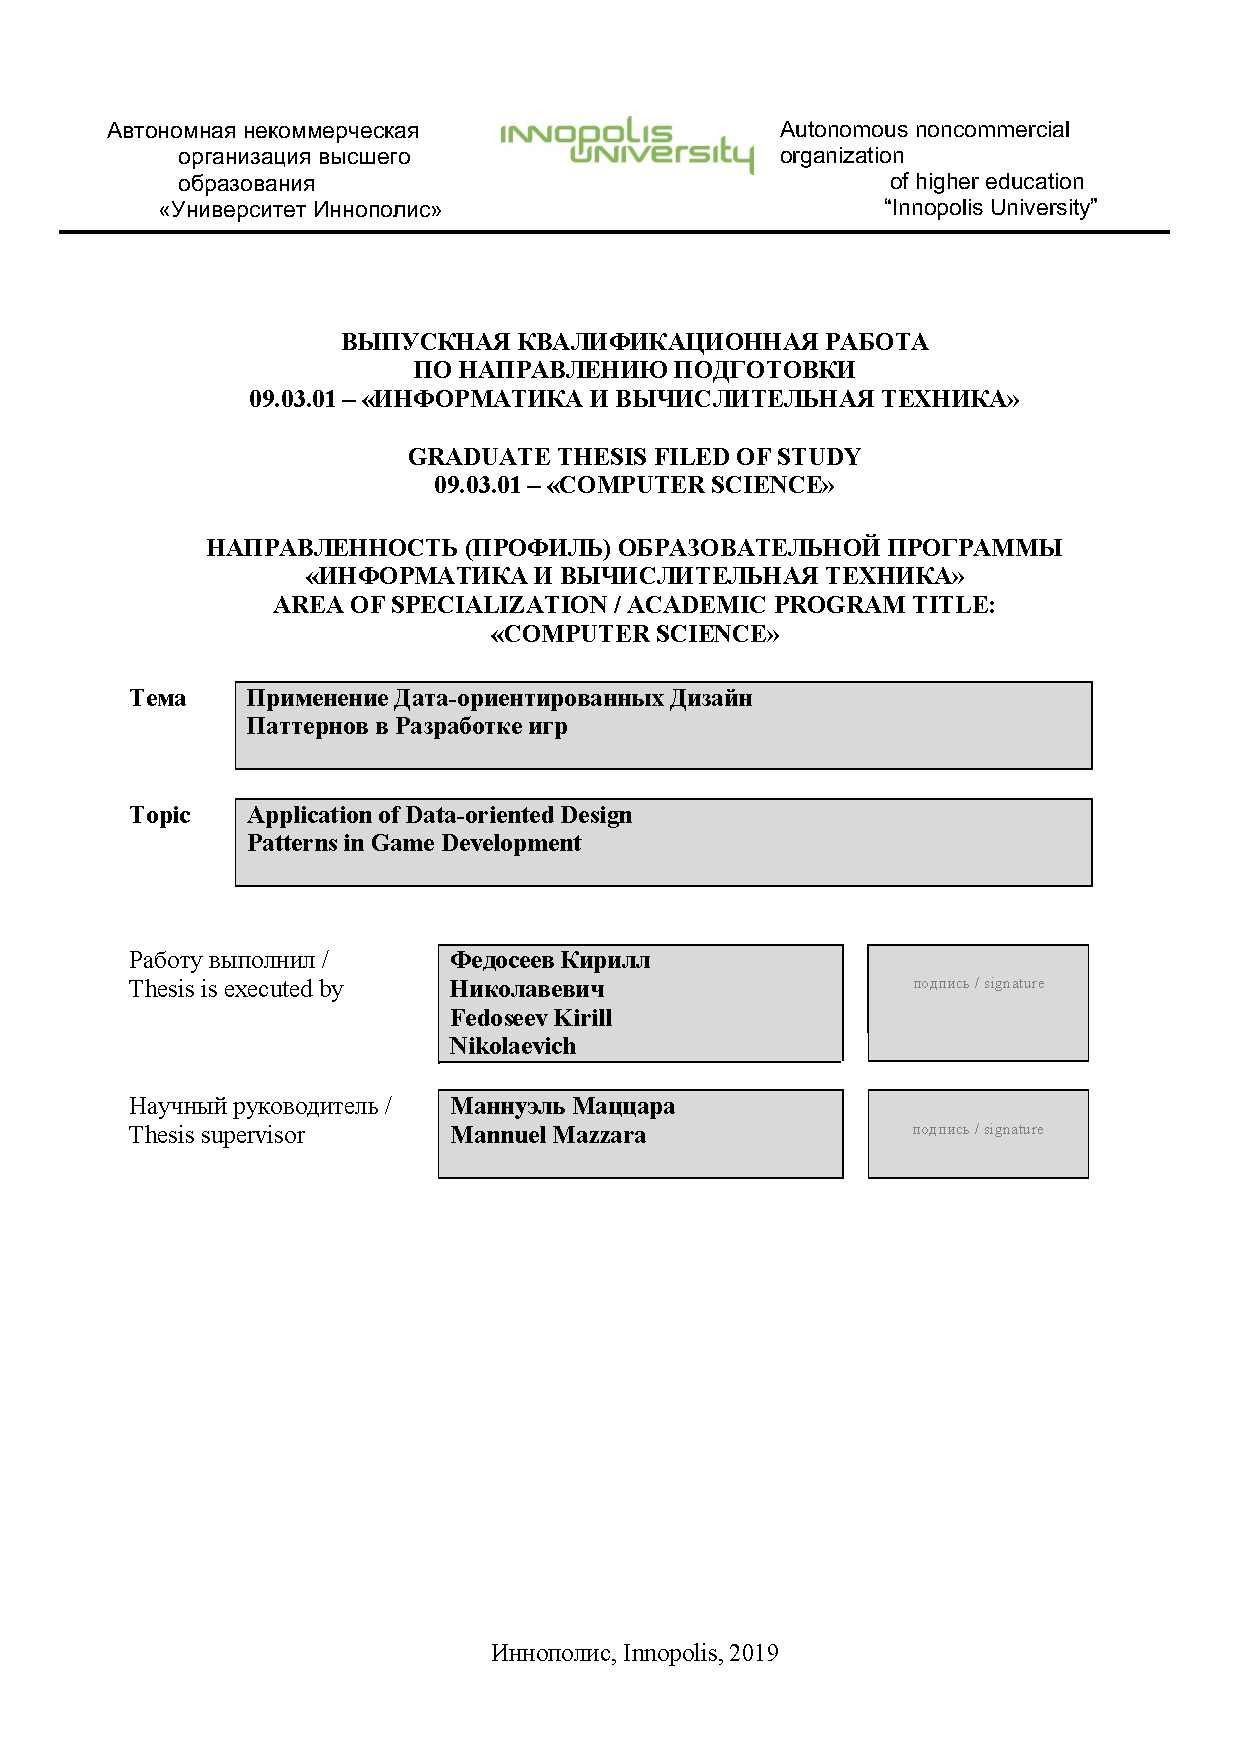
\includepdf[pages=-]{titles/BS.pdf}
\setcounter{page}{5}
\thispagestyle{empty}
\mbox{}

\tableofcontents
\listoftables
\listoffigures

\newpage
\begin{abstract}


\end{abstract}
\chapter{Introduction}
\label{chap:intro}
\chaptermark{Optional running chapter heading}


\section{Context}
\label{sec:context}
Data-oriented design (DOD) is gaining popularity in the game development, and is an alternative approach to more traditional Object-oriented design (OOD). 

DOD is a software design approach aiming at efficient usage of the CPUs cache. The approach is to focus not on relations between data as in OOD, but on the layout of it directed on separating and sorting fields according to when they are needed, and to think about transformations of data.

The main advantage of DOD, is that it allows design and develop  game engines which efficiency utilize devices with multicore processor hardware through uniformly spreading the CPUs load over multiple threads, which is not possible using object oriented paradigm. This, in turn, grants the games built using DOD a more optimized resource utilization and performance, that are so critical in game development. In particular, games, which is OOD,  usually use one main thread for approximately  80\% of all CPU tasks, that is not good in nowadays, when most of devices have multicore CPU.

Despite its advantages and growing popularity, application of DOD in game development has not been subject of many academic research papers. Moreover, transformation of existing game projects from OO paradigm to DO has not been examined either. The question that arises is how can a development team transform a game project from OO to DO and what are the fundamental problems? Are there design patterns and templates to do it in a more effective way?

\section{Objectives}
\label{sec:objectives}

This paper aims to provide an introduction to DOD in comparison with OOD by describing the two paradigms and the key difference between them. Following the introductory notes on both approaches, the paper will provide an overview of some of the existing DOD design patterns, and examine their application in the context of several real game development projects. In particular, a transformation from OOD to DOD will be performed for several mobile games made on Unity platform, that was chosen since it fits the use case for the planned work. Unity includes Entity Component System (ECS) framework, that allows to utilize multithreading and can be used for implementation of DOD principles and patterns that emerged in the industry. The results of transformation and implementation of each pattern in the context of the mobile game projects will be analyzed. 

Based on the analysis, the general applicability of the patterns to other projects will be discussed together with the potential advantages and disadvantages of using the patterns to perform transformations of software components from OO to DO design. An important question to be considered is what the criteria are for a team to decide whether to migrate from OOD to DOD in a given project. Also, the discussion will touch upon other factors and possible trade-offs connected to the use of DOD as opposed to OOD, such as team composition, company context and culture, and developer preferences.


\section{Expected Outcomes}
\label{sec:objectives}
This thesis will contain at the end:


\begin{itemize}
\item Short explanation about DOD, in particular Unity ECS including references to more deep sources. 
\item Table with analysis in SWOT manner such things related to games
\begin{itemize}
\item overall performance
\item maintainability
\item testability
\item entry level for developers and others

\end{itemize}
\item From 3 to 5 patterns, design principles or techniques mapped on real game OO structure with advantages and disadvantages analysis.
\item List of materials with summaries.
\end{itemize}

The content will aim to fulfil objectives and answer the main question raised in the introductory part and the objectives.

\section{Milestones}
\label{sec:objectives}

\textbf{Fall}  \newline
Deliverable 0 – Project overleaf: due by 16.09.2019\newline
Deliverable 1 – Explanation about DOD and ECS:  due by 15.10.2019\newline
Deliverable 2 – Analysis of using DOD in games:  due by 15.11.2019\newline
Deliverable 3 – Sketch of some cases in transforming from OO to DO structure of real game: due by 15.12.2019\newline
 \newline
\textbf{Spring} \newline
Deliverable 4 – Collected feedback about sketches(del 3): due by 1.2.2020\newline
Deliverable 5 – Complete 3-5 cases of transformation from OO to DO structures: due by 15.3.2020\newline
Deliverable 6 – Full thesis draft: due by 31.3.2020\newline
Deliverable 7 – Final demo and presentation: due by 15.4.2020\newline
 \newline
\textbf{Summer}  \newline
Deliverable 8 – Final Thesis and abstract: deadline decided by DoE\newline
Deliverable 9 – Presentation to commission: deadline decided by DoE\newline





\include{chapters/chapter1}
\chapter{Literature Study and Theory}
\label{chap:lr}
\chaptermark{Second Chapter Heading}


\Blindtext[2]

\section{Computers' Memory}
\Blindtext[1]
\section{DOD}
\Blindtext[1]
\section{OOP}
\Blindtext[1]
\section{Component Over Inheritance}
\Blindtext[1]
\section{Unity ECS}
\Blindtext[1]

\include{chapters/сhapter3_FuncSpec}
\include{chapters/chapter3_Mat&Meth}
\chapter{Materials and Methods}
\label{chap:met}


\ldots

Referencing other chapters \ref{chap:lr}, \ref{chap:met}, \ref{chap:impl}, \ref{chap:eval} and \ref{chap:conclusion}

\ldots
\chapter{Implementation}
\label{chap:impl}


\ldots

\chapter{Evaluation and Discussion}
\label{chap:eval}


\ldots



%% REFERENCES
\bibliographystyle{apalike}
\bibliography{thesis}
\appendix
\chapter{Extra Stuff}
\blindtext

\chapter{Even More Extra Stuff}
\blindtext
\end{document}

